

\section{Introduction}
\index{Scenario Damage}
The scenario damage calculator can be employed to estimate the distribution of damage due to a single earthquake, for a spatially distribute building portfolio. Similarly to what has been described for the scenario risk calculator, a finite \gls{rupture} should be used to derive sets of \glspl{groundmotionfield}. 

In this calculator, each \gls{groundmotionfield} is combined with a \gls{fragility model} (discrete or continuous), in order to compute the fractions of buildings in each damage state. These fractions are calculated based on the difference in probabilities of exceedance between consecutive limit state curves at a given intensity measure level. This process is repeated for each \gls{groundmotionfield}, leading to a list of fractions for each \gls{asset}. These results can then be multiplied by the respective number or area of buildings in order to obtain the absolute building damage distribution.

\section{Calculation Steps}

\begin{enumerate}
\item For each \gls{groundmotionfield}, the intensity measure level at the location of the \gls{asset} is used to derive the
fraction of buildings in each damage state. In order to do so, the distance between each pair of consecutive limit states is calculated. This process is illustrated in Figure \ref{fig:FragilityProcess}, using a continuous \gls{fragility function}.

\begin{figure}[ht]
\centering
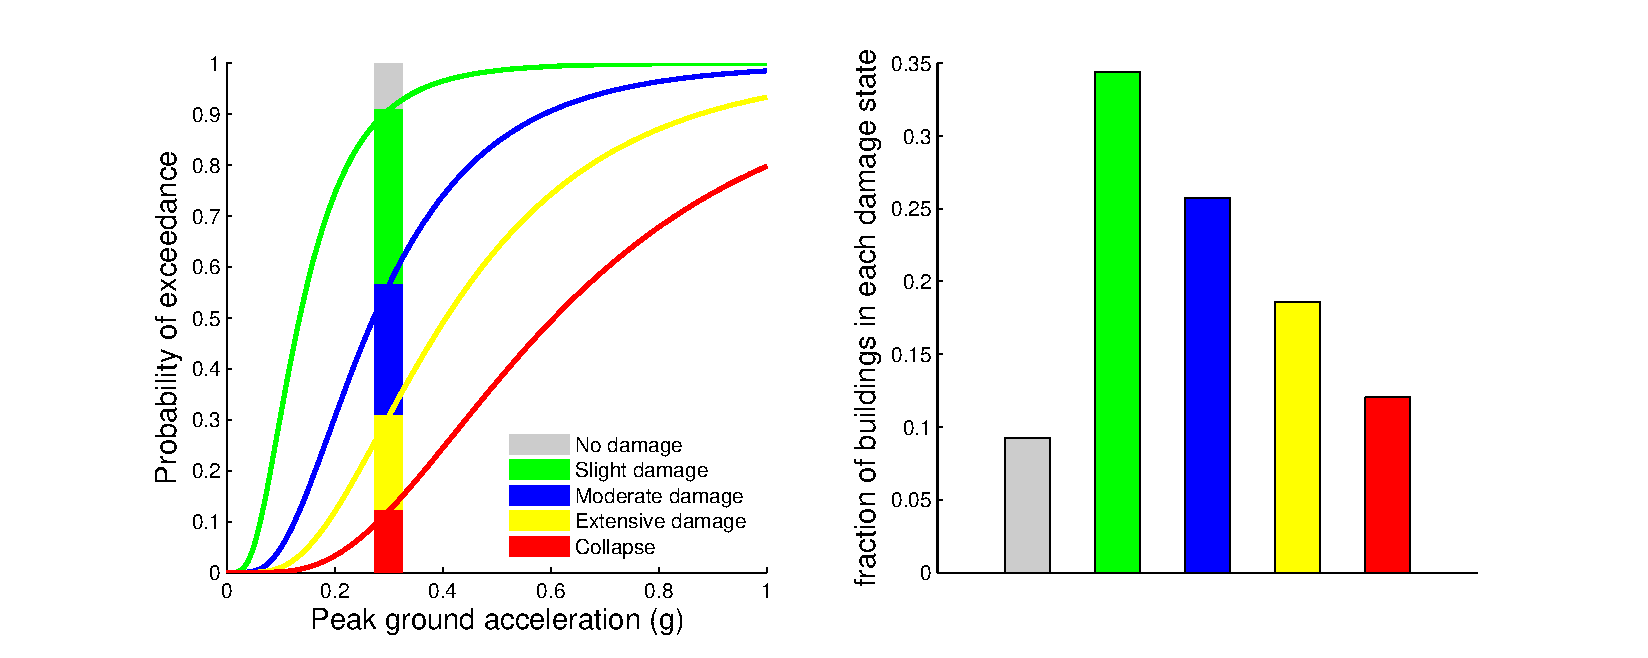
\includegraphics[width=14cm,height=5cm]{./figures/risk/Fragility_process.eps}
\caption{Representation of the fractions of building in each damage states, for a given intensity measure level (0.3 g).}
\label{fig:FragilityProcess}
\end{figure}

When a continuous \gls{fragility function} is used for the calculations, the fractions of building in each damage state are calculated using the analytical expression of the lognormal cumulative distribution functions. On the other hand, if a discrete \gls{fragility function} was chosen, these fractions are computed using linear interpolation between the pair of points either side of the intensity measure level.

\item Step 1 is repeated for each \gls{groundmotionfield}, leading to a list of fractions (one per damage state), for each \gls{asset}. From this list of values, the mean ($E[FR]$) and standard deviation ($SD[FR]$) for each fraction can be estimated using the following formulae:

\begin{equation}
E[FR]=\frac{\sum^m_{n=1}FR_n|IML}{m}
\end{equation}

\begin{equation}
SD[FR]=\sqrt{  \frac{1}{m}\sum_{n=1}^m{(FR_n-E[FR])^2} }
\end{equation}
 
Where $m$ stands for the number of \glspl{groundmotionfield} simulated. 

\item These fractions of buildings in each damage state can be multiplied by the quantity of the respective asset, leading to the mean and standard deviation of the number or area of buildings in each damage state (see Figure \ref{fig:AssetDis}). 

\item This calculator is also capable of estimating the aggregated number or area of buildings from the same \gls{taxonomy} in each damage state (see Figure \ref{fig:TaxDis}). In order to do so, for each \gls{groundmotionfield}, the absolute quantity of buildings in each damage state is calculated, and aggregated according to their \gls{taxonomy}. After processing all the \glspl{groundmotionfield}, the associated statistics for each building \gls{taxonomy} are calculated according to the formulae described in Step 2.

\item The total damage distribution is also calculated, by summing the quantity of buildings in each damage state, across all the \glspl{asset} existing in the building portfolio. This calculation will lead to a single damage distribution, represented by a mean and standard deviation for each damage state (see Figure \ref{fig:TotalDis}).

\end{enumerate}

\section{Calculator Output}
The output of the Scenario Damage Calculator currently comprises damage distributions at three levels: per \gls{asset}, per building \gls{taxonomy} and total. In addition, with this calculator, is it also possible to extract collapse maps, which contain the spatial distribution of the number or area of collapsed buildings throughout the region of interest (see Figure \ref{fig:CollapseMap}). In the figures shown herein, examples of the outputs are depicted for a scenario event of magnitude 7.0Mw in the central region of Nepal.

\begin{figure}[ht]
\centering
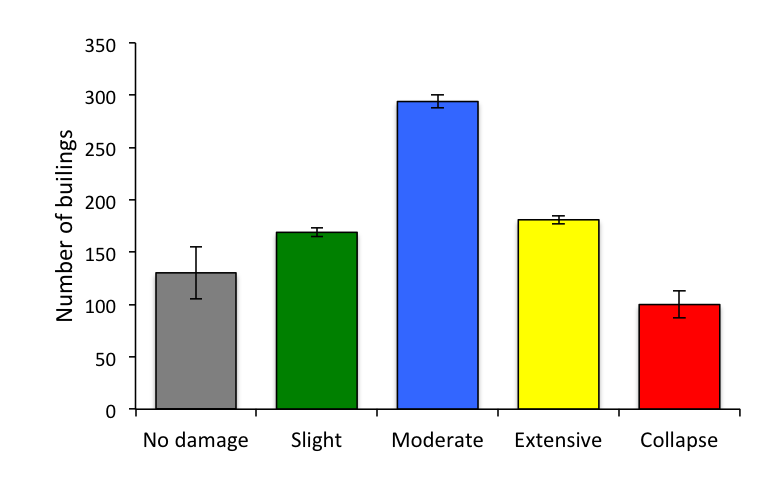
\includegraphics[width=8cm,height=5cm]{./figures/risk/AssetDisaggregation.eps}
\caption{Damage distribution for a single asset.}
\label{fig:AssetDis}
\end{figure} 

\begin{figure}[ht]
\centering
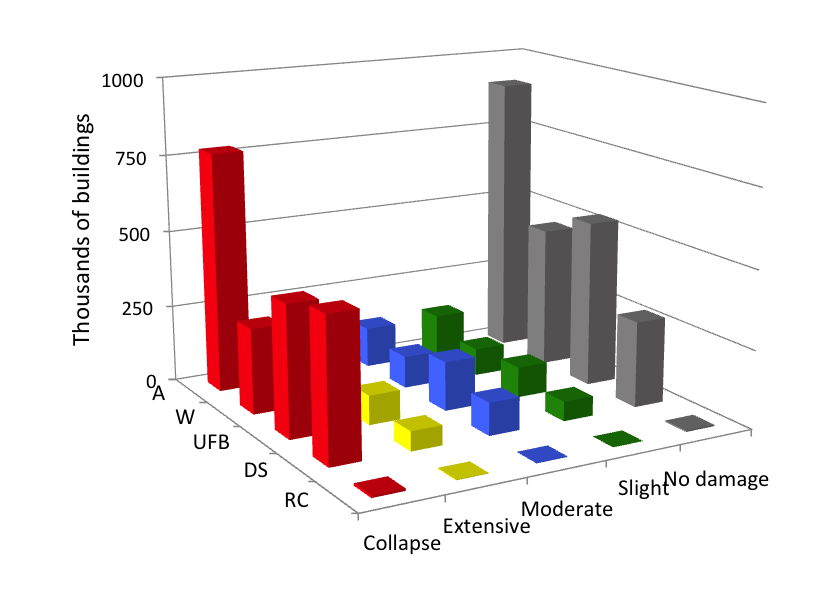
\includegraphics[width=8cm,height=5cm]{./figures/risk/TaxonomyDisaggregation.eps}
\caption{Damage distribution according to the building taxonomy.}
\label{fig:TaxDis}
\end{figure} 

\begin{figure}[ht]
\centering
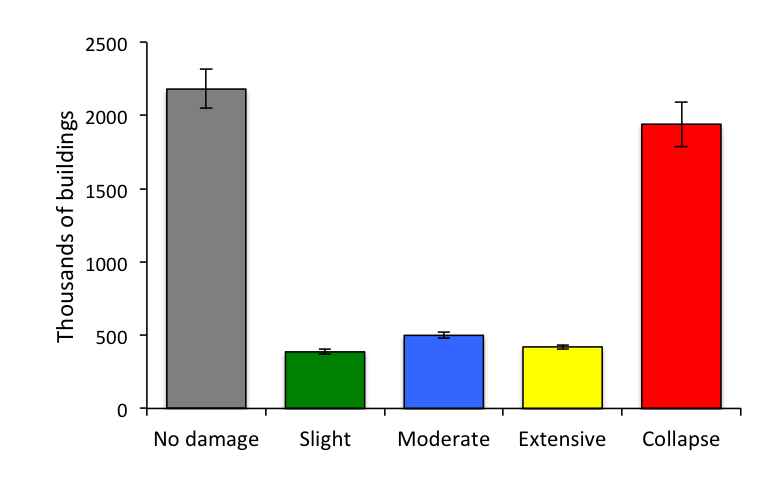
\includegraphics[width=8cm,height=5cm]{./figures/risk/TotalDis.eps}
\caption{Damage distribution of the whole building portfolio.}
\label{fig:TotalDis}
\end{figure} 

\begin{figure}[ht]
\centering
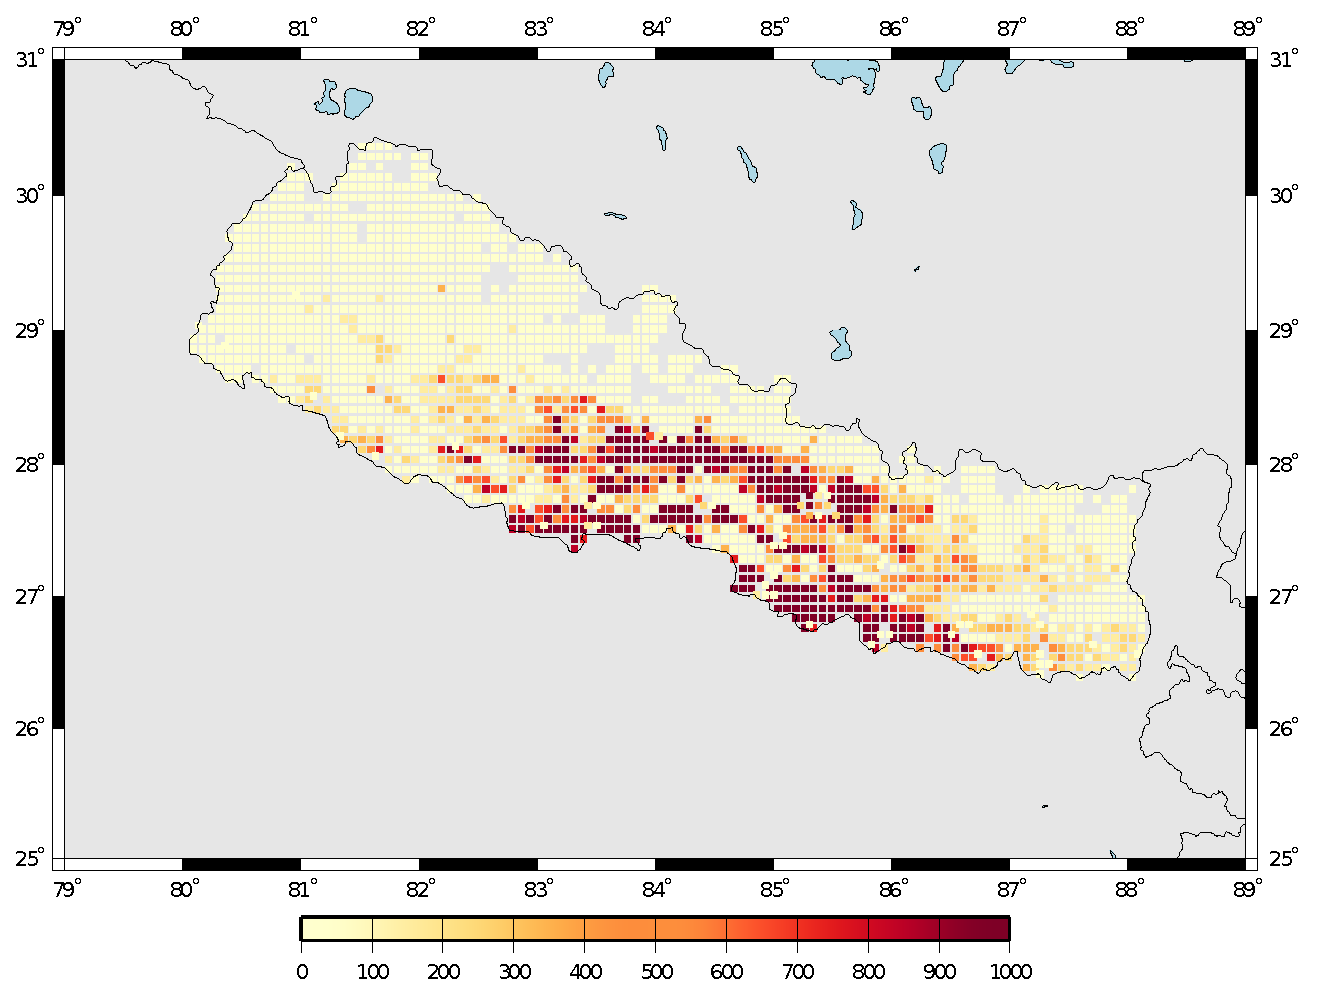
\includegraphics[width=12cm,height=7cm]{./figures/risk/CollapseMap.eps}
\caption{Collapse map considering the whole building portfolio.}
\label{fig:CollapseMap}
\end{figure} 